%iffalse
\let\negmedspace\undefined
\let\negthickspace\undefined
\documentclass[journal,12pt,twocolumn]{IEEEtran}
\usepackage{cite}
\usepackage{amsmath,amssymb,amsfonts,amsthm}
\usepackage{algorithmic}
\usepackage{graphicx}
\usepackage{textcomp}
\usepackage{xcolor}
\usepackage{txfonts}
\usepackage{listings}
\usepackage{multicol}
\usepackage{enumitem}
\usepackage{mathtools}
\usepackage{gensymb}
\usepackage{comment}
\usepackage[breaklinks=true]{hyperref}
\usepackage{tkz-euclide} 
\usepackage{listings}
\usepackage{gvv}                                        
%\def\inputGnumericTable{}                                 
\usepackage[latin1]{inputenc}                                
\usepackage{color}                                            
\usepackage{array}                                            
\usepackage{longtable}                                       
\usepackage{calc}                                             
\usepackage{multirow}                                         
\usepackage{hhline}                                           
\usepackage{ifthen}                                           
\usepackage{lscape}
\usepackage{tabularx}
\usepackage{array}
\usepackage{float}


\newtheorem{theorem}{Theorem}[section]
\newtheorem{problem}{Problem}
\newtheorem{proposition}{Proposition}[section]
\newtheorem{lemma}{Lemma}[section]
\newtheorem{corollary}[theorem]{Corollary}
\newtheorem{example}{Example}[section]
\newtheorem{definition}[problem]{Definition}
\newcommand{\BEQA}{\begin{eqnarray}}
\newcommand{\EEQA}{\end{eqnarray}}
\newcommand{\define}{\stackrel{\triangle}{=}}
\theoremstyle{remark}
\newtheorem{rem}{Remark}

% Marks the beginning of the document
\begin{document}
\bibliographystyle{IEEEtran}
\vspace{3cm}

\title{Assignment-1}
\author{AI24BTECH11036- Shreedhanvi Yadlapally}
\maketitle
\newpage
\bigskip
\section{MCQ's with Single Correct Answer}
\begin{enumerate}
	\item The locus of $z$ which lies in the shaded region (excluding the boundaries) is best represented by
\\

\hfill{(2005S)}\\
	        \begin{figure}[ht]
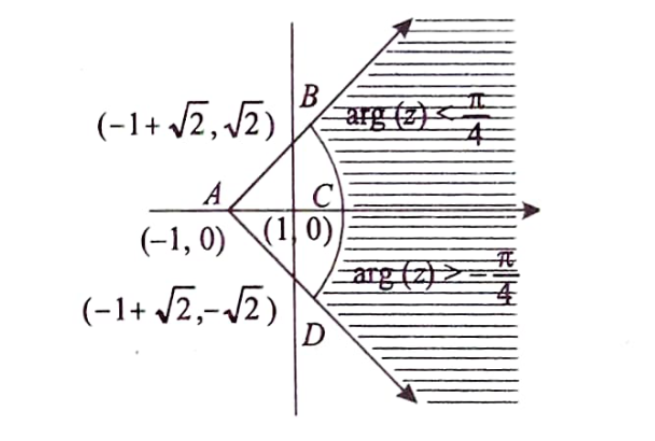
\includegraphics[scale=0.2]{Figure/Screenshot_20240807-085214}
		\end{figure}
		%insert graph here
\begin{enumerate}[label=(\alph*)]
\item $z:\abs{z+1}>2$ and  $\abs{arg(z-1)}<\frac{\pi}{4}$
\item $z:\abs{z-1}>2$ and $\abs{arg(z-1)}<\frac{\pi}{4}$
\item $z:\abs{z+1}<2$ and $\abs{arg(z+1)}<\frac{\pi}{2}$
\item $z:\abs{z-1}<2$ and $\abs{arg(z+1)}<\frac{\pi}{2}$
\end{enumerate}

\item $a,b,c$ are integers, not all simultaneously equal and $\omega$ is the cube root of unity ($\omega \neq 1$), then the minimum value of $\abs{a+b\omega+c\omega^{2}l}$ is?         \\

        \hfill{(2005S)}
		\begin{multicols}{4}
\begin{enumerate}[label=(\alph*)]
	\item $0$
	\item $1$
	\item $\frac{\sqrt{3}}{2}$
	\item $\frac{1}{2}$
\end{enumerate}
                 \end{multicols}

\item Let $\omega=\frac{-1}{2}+i\frac{\sqrt{3}}{2}$,then the value of det?\\
	\begin{align}
	\begin{vmatrix}
	1     &1               &1            \\
	1     &-1-\omega^{2}   &\omega^{2}   \\
	1     &\omega^{2}      &\omega^{4}
        \end{vmatrix}
	\end{align}
	\hfill{(2002- 2M)}
		\begin{multicols}{2}
\begin{enumerate}[label=(\alph*)]
	\item $3\omega$
	\item $3\omega\brak{\omega-1}$
	\item $3\omega^{2}$
	\item $3\omega\brak{1-\omega}$
\end{enumerate}
		\end{multicols}

\item If $\frac{w-\overline{w}z}{1-z}$ is purely real where $w=\alpha+i\beta, \beta \neq 0$ and $z \neq 1$. Then the set of values of $z$ is?                     \\

	\hfill{(2006-3M)}
		\begin{multicols}{2}
\begin{enumerate}[label=(\alph*)]
	\item {$z:\abs{z}=1$}
	\item {$z:z= \overline{z}$}
	\item {$z:z \neq 1 $}
	\item {$z:\abs{z}=1, z\neq1$}
\end{enumerate}
		\end{multicols}

\item A man walks a distance of 3 units from the origin towards the north-east (N 45\degree E) direction. From there, he walks a distance of 4 units towards the northwest (N 45\degree W) direction to reach a poit $P$. The position of $P$ in the Argand Plane is \hfill{(2007-3M)}
	\begin{multicols}{2}
\begin{enumerate}[label=(\alph*)]
	\item $3e^{\frac{i\pi}{4}}+4i$
	\item $\brak{3-4i}e^{\frac{i\pi}{4}}$
	\item $\brak{4+3i}e^{\frac{i\pi}{4}}$
	\item $\brak{3+4i}e^{\frac{i\pi}{4}}$
\end{enumerate}
	\end{multicols}

\item If $\abs{z}=1$ and $z\neq\pm1$, then all the values of $\frac{z}{1-z^{2}}$ lie on \hfill{(2007-3M)}
\begin{enumerate}[label=(\alph*)]
	\item a line not passing through origin
	\item $\abs{z}=\sqrt{2}$
	\item the x-axis
	\item the y-axis
\end{enumerate}

\item A particle $P$ starts from the point $z_{0}=1+2i$, where $i=\sqrt{-1}$. It moves horizontally away from origin by 5 units and then vertically away from origin by 3 units to reach apoint $z_{1}$. From $z_{1}$, the particle moves $\sqrt{2}$ units in the direction of the vector $\hat{i}+\hat{j}$ and then it moves through an angle $\frac{\pi}{2}$ in anticlockwise direction on a circle with centre at origin, to reach a point $z_{2}$. The point $z_{2}$ is given by \hfill{(2008)}
	\begin{multicols}{2}
\begin{enumerate}[label=(\alph*)]
	\item $6+7i$
	\item -$7+6i$
	\item $7+6i$
	\item -$6+7i$
\end{enumerate}
	\end{multicols}

\item Let $z=\cos\theta+i\sin\theta$. Then the value of $\sum_{m=1} ^{15}$ Im($z^{2m-1}$) at $\theta=2\degree$ is \hfill{(2009)}
	\begin{multicols}{4}
\begin{enumerate}[label=(\alph*)]
	\item $\frac{1}{\sin 2\degree}$
	\item $\frac{1}{3\sin 2\degree}$
	\item $\frac{1}{2\sin 2\degree}$
	\item $\frac{1}{4\sin 2\degree}$
\end{enumerate}
	\end{multicols}

\item Let $z=x+iy$ be a complex number where $x$ and $y$ are integers. Then the area of the rectangle whose vertices are the roots of the equation: $z\overline{z}^{3}+\overline{z}z^{3}=350$ is \hfill{(2009)}
	\begin{multicols}{4}
\begin{enumerate}[label=(\alph*)]
	\item 48
	\item 32
	\item 40
	\item 80
\end{enumerate}
	\end{multicols}

\item Let $z$ be a complex number such that the imaginary part of z is non-zero and $a=z^{2}+z+1$ is real. The $a$ cannot take the value \hfill{(2012)}
	\begin{multicols}{4}
\begin{enumerate}[label=(\alph*)]
	\item -1
	\item $\frac{1}{3}$
	\item $\frac{1}{2}$
	\item $\frac{3}{4}$
\end{enumerate}
	\end{multicols}

\item Let complex numbers $\alpha$ and $\frac{1}{\overline{\alpha}}$ lie on circles $(x-x_{0})^{2}+(y-y_{0})^{2}=r^{2}$ and $(x-x_{0})^{2}+(y-y_{0})^{2}=4r^{2}$ respectively. If $z_{0}=x_{0}+iy_{0}$ satisfies the equatio  $2\abs{z_{0}} ^{2}=r^{2}+2$, the $\abs{\alpha}$= \hfill{(2013)}
	\begin{multicols}{4}
\begin{enumerate}[label=(\alph*)]
	\item $\frac{1}{\sqrt{2}}$
	\item $\frac{1}{2}$
	\item $\frac{1}{\sqrt{7}}$
	\item $\frac{1}{3}$
\end{enumerate}
	\end{multicols}

\item Let $S$ be the set of all complex numbers $z$ satisfying $\abs{z-2+i}\geq\sqrt{5}$. If the complex number $z_{0}$ is such that $\frac{1}{\abs{z_{0}-1}}$ is the maximum of the set  $\cbrak{\frac{1}{|z-1|} : z \in S}$, then the principal argument of $\frac{4-z_{0}-\overline{z_{0}}}{z_{0}-\overline{z_{0}}+2i}$ is  \hfill{(2019)}
	\begin{multicols}{4}
\begin{enumerate}[label=(\alph*)]
	\item $\frac{\pi}{4}$
	\item $\frac{3\pi}{4}$
	\item $\frac{\pi}{2}$
	\item -$\frac{\pi}{2}$
\end{enumerate}
	\end{multicols}

\end{enumerate}

\section{ MCQ's with One or More than One Correct}
\begin{enumerate}
	\item If $z_{1}=a+ib$ and $z_{2}=c+id$ are complex numbers such that $\abs{z_{1}}=\abs{z_{2}}=1$ and Re($z_{1}\overline{z_{2}}$)=0, then the pair of complex numbers $w_{1}=a+ic$ and $w_{2}=b+id$ satisfies \hfill{(1985 - 2 Marks)}
		\begin{multicols}{2}
\begin{enumerate}[label=(\alph*)]
	\item $\abs{w_{1}}=1$
	\item $\abs{w_{2}}=1$
	\item Re($w_{1}\overline{w_{2}}$)=0
	\item none of these.
\end{enumerate}
		\end{multicols}

\item Let $z_{1}$ and $z_{2}$ be complex numbers such that $z_{1}\neq z_{2}$ and $\abs{z_{1}}=\abs{z_{2}}$. If $z_{1}$ has positive real part and $z_{2}$ has negative imaginary part, then $\frac{z_{1}+z_{2}}{z_{1}-z_{2}}$ may be \hfill{(1986 - 2 Marks)}
	\begin{multicols}{2}
\begin{enumerate}[label=(\alph*)]
	\item zero
	\item real and positive
	\item real and negative
	\item purely imaginary
	\item none of the these.
\end{enumerate}
	\end{multicols}

\item If $z_{1}$ and $z_{2}$ are two non-zero complex numbers such that $\abs{z_{1}+z_{2}}=\abs{z_{1}}+\abs{z_{2}}$, then arg$z_{1}$ - arg$z_{2}$ is equal to \hfill{(1987 - 2 Marks)}
	\begin{multicols}{4}
\begin{enumerate}[label=(\alph*)]
	\item -$\pi$
	\item -$\frac{\pi}{2}$
        \item 0
        \item $\frac{\pi}{2}$
	\item $\pi$
\end{enumerate}
	\end{multicols}

\item The value of $\sum_{k=1} ^{6} (\sin \frac{2\pi k}{7}-i\cos \frac{2\pi k}{7})$ is                        \\

	\hfill{(1987 - 2 Marks)}
		\begin{multicols}{4}
\begin{enumerate}[label=(\alph*)]
	
	\item -1
	\item 0
	\item -$i$
	\item $i$
	\item None
\end{enumerate}
		\end{multicols}

\end{enumerate}

\renewcommand{\thefigure}{\theenumi}
\renewcommand{\thetable}{\theenumi}


\end{document}

